\documentclass[11pt,a4paper]{article}
\usepackage[margin=2.2cm]{geometry}
\usepackage{amsmath,amssymb}
\usepackage{graphicx}
\usepackage{float}
\usepackage{array}
\usepackage{booktabs}
\usepackage{multirow}
\usepackage{tabularx}
\usepackage{longtable}
\usepackage{hyperref}
\usepackage{enumitem}
\usepackage{setspace}
\usepackage{caption}
\usepackage{xcolor}
\usepackage{titlesec}
\usepackage{makecell}
\usepackage[T1]{fontenc}
\usepackage[utf8]{inputenc}
\newcolumntype{Y}{>{\centering\arraybackslash}X}

\graphicspath{{Group12_Assignment1_code/outputs/classification_ls/logistic/}{Group12_Assignment1_code/outputs/classification_ls/tanh/}{Group12_Assignment1_code/outputs/classification_nls/logistic/}{Group12_Assignment1_code/outputs/classification_nls/tanh/}{Group12_Assignment1_code/outputs/regression_univariate/}{Group12_Assignment1_code/outputs/regression_bivariate/}}

\titleformat{\section}{\normalfont\Large\bfseries}{\thesection}{1em}{}
\titleformat{\subsection}{\normalfont\large\bfseries}{\thesubsection}{1em}{}
\titleformat{\subsubsection}{\normalfont\normalsize\bfseries}{\thesubsubsection}{1em}{}

\begin{document}
\thispagestyle{empty}
\begin{center}
    \vspace*{1cm}
    {\LARGE \textbf{Perceptron-Based Classification and Regression}}\\[0.5cm]
    {\large CS601T: Deep Learning -- Programming Assignment I}\\[1.2cm]
    {\large \textbf{Group 12}}\\[0.7cm]
    {\itshape Submitted by}\\[0.3cm]
    {\large \textbf{Dattaraj Balkrishna Saudagar} (Roll No.: CS24BT037)}\\
    {\large \textbf{Onkar Avinash Mulje} (Roll No.: CS24BT059)}\\
    {\large \textbf{Nimitt Jain} (Roll No.: CS24BT048)}\\[1.2cm]
    {\large \textbf{Department of Computer Science and Engineering}}\\
    {\large \textbf{Indian Institute of Technology Dharwad}}\\[0.5cm]
    {\large August 2026}
\end{center}
\clearpage

\tableofcontents
\clearpage

\section*{Abstract}
This report presents the design, implementation, and evaluation of a single-layer perceptron for both classification and regression tasks, implemented entirely from scratch (without using any perceptron, neural network, or gradient-descent library). For classification, perceptrons with logistic and tan-hyperbolic activation functions were trained using a one-against-one strategy on a linearly separable (LS) and a non-linearly separable (NLS) three-class, two-dimensional dataset. For regression, a perceptron with a linear activation function was trained on a univariate and a bivariate dataset. All models were trained using the online gradient-descent learning rule. Performance is reported using confusion matrices, accuracy, class-wise and mean precision/recall/F-measure for classification, and RMSE / \%RMSE for regression, all computed using custom implementations. Results show perfect separation on the linearly separable data and the expected performance degradation on the non-linearly separable and non-linear regression data, illustrating the fundamental limitation of a single linear decision boundary.
\clearpage

\section{Introduction}
The perceptron is the simplest artificial neuron: it computes a weighted sum of its inputs (the net input), passes this sum through a non-linear activation function, and produces a single scalar output. Despite its simplicity, the perceptron is the fundamental building block of larger neural networks, and understanding its learning rule and its limitations motivates the need for multi-layer architectures.

This assignment implements the perceptron learning algorithm from first principles and applies it to two kinds of tasks:

\textbf{Classification:} a 3-class, 2-dimensional problem is solved using a one-against-one ensemble of perceptrons, once with a logistic activation function and once with a tan-hyperbolic (tanh) activation function, on two datasets -- one linearly separable (LS) and one non-linearly separable (NLS).

\textbf{Regression:} a perceptron with a linear activation function is trained to predict a continuous target from a univariate input and, separately, from a bivariate input.

In both cases the weights are updated using the online (per-sample) gradient-descent rule that minimizes the mean-squared error between the perceptron's output and the target, and every evaluation metric (confusion matrix, precision, recall, F-measure, RMSE, \%RMSE) is implemented from scratch as required by the assignment.
\clearpage

\section{Methodology}
\subsection{Perceptron Model}
Each perceptron computes a net input as a weighted sum of the input features plus a bias, and applies an activation function $f$ to obtain its output $o=f(\text{net})$:
\[
\mathrm{net} = \sum_{i=1}^{d} w_i x_i + b = \mathbf{w}^T\mathbf{x} + b
\]

Three activation functions are used in this assignment:

\textbf{Logistic (sigmoid)} -- used for classification, output in $(0,1)$:
\[
f(\mathrm{net}) = \frac{1}{1+e^{-\mathrm{net}}}, \qquad f'(\mathrm{net}) = f(\mathrm{net})\,(1-f(\mathrm{net}))
\]

\textbf{Tan-hyperbolic (tanh)} -- used for classification, output in $(-1,1)$:
\[
f(\mathrm{net}) = \tanh(\mathrm{net}), \qquad f'(\mathrm{net}) = 1 - f(\mathrm{net})^2
\]

\textbf{Linear} -- used for regression, output unbounded:
\[
f(\mathrm{net}) = \mathrm{net}, \qquad f'(\mathrm{net}) = 1
\]

\subsection{Gradient-Descent Learning Rule}
Training minimizes the mean-squared error between target $t$ and output $o$ over the $N$ training samples:
\[
E = \frac{1}{2N}\sum_{k=1}^{N}(t_k-o_k)^2
\]

Differentiating this error with respect to each weight gives the online (per-sample) gradient-descent update rule, applied after every training example with learning rate $\eta$:
\[
w_i \leftarrow w_i + \eta\,(t-o)\,f'(\mathrm{net})\,x_i, \qquad b \leftarrow b + \eta\,(t-o)\,f'(\mathrm{net})
\]

For the logistic and tanh activations the targets are encoded as $\{0,1\}$ and $\{-1,+1\}$ respectively; for the linear activation used in regression, $f'(\mathrm{net})=1$ and the target is the real-valued output directly. Weights are initialized to small random values and the dataset order is reshuffled every epoch.

\subsection{One-Against-One Multi-Class Strategy}
Since a single perceptron only produces a binary decision, the 3-class classification problem is solved with three pairwise perceptrons: Class1-vs-Class2, Class1-vs-Class3, and Class2-vs-Class3, each trained only on the samples belonging to that pair of classes. At prediction time, all three pairwise classifiers vote for one of their two classes, and the class with the majority of votes is chosen as the final label; ties (possible when each classifier votes for a different class) are broken using the sum of the winning classifiers' confidence scores ($|\text{output}-\text{decision threshold}|$).

\subsection{Evaluation Metrics (implemented from scratch)}
For classification, a confusion matrix $CM$ is built by counting true-label vs. predicted-label pairs on the test set. From it, per-class precision and recall are computed as:
\[
\mathrm{Precision}_j = \frac{CM_{jj}}{\sum_i CM_{ij}}
\]
\[
\mathrm{Recall}_i = \frac{CM_{ii}}{\sum_j CM_{ij}}
\]

and the per-class F-measure is their harmonic mean:
\[
F_i = \frac{2\,\mathrm{Precision}_i\,\mathrm{Recall}_i}{\mathrm{Precision}_i+\mathrm{Recall}_i}
\]

Accuracy is the fraction of correctly classified test samples, and the mean precision, mean recall and mean F-measure are simple averages of the per-class values. For regression, the root-mean-squared error and percentage RMSE (RMSE normalized by the mean of the target values) are used:
\[
\mathrm{RMSE} = \sqrt{\frac{1}{N}\sum_{k=1}^{N}(t_k-o_k)^2}
\]
\[
\%\mathrm{RMSE} = \frac{\mathrm{RMSE}}{\overline{t}}\times 100
\]
\clearpage

\section{Experimental Setup}
\subsection{Datasets}
\begin{table}[H]
\centering
\renewcommand{\arraystretch}{1.3}
\begin{tabular}{|p{0.22\textwidth}|p{0.25\textwidth}|p{0.17\textwidth}|p{0.28\textwidth}|}
\hline
\rowcolor{blue!60}\color{white}\textbf{Task} & \color{white}\textbf{Dataset} & \color{white}\textbf{Size} & \color{white}\textbf{Description} \\
\hline
Classification & LS (Dataset 1) & $3\times500=1500$ & 2-D, linearly separable \\
\hline
Classification & NLS (Dataset 2) & $3\times500=1500$ & 2-D, non-linearly separable \\
\hline
Regression & Univariate (Dataset 1) & 1000 & 1-D input, 1-D output \\
\hline
Regression & Bivariate (Dataset 2) & 10200 & 2-D input, 1-D output \\
\hline
\end{tabular}
\caption*{Dataset summary used in the experiments.}
\end{table}

\subsection{Train / Test Split}
For every dataset, each class (classification) or the whole dataset (regression) is split into 70\% training data and 30\% test data using a fixed random seed. The split is performed exactly once by a dedicated data-preparation step and the resulting indices are cached to disk; every subsequent training run (for any activation function or model configuration) loads this same cached split, so the train/test partition never changes when switching between models.

\subsection{Hyperparameters}
\begin{table}[H]
\centering
\renewcommand{\arraystretch}{1.3}
\begin{tabular}{|p{0.45\textwidth}|p{0.27\textwidth}|p{0.22\textwidth}|}
\hline
\rowcolor{blue!60}\color{white}\textbf{Experiment} & \color{white}\textbf{Learning Rate} & \color{white}\textbf{Max Epochs} \\
\hline
Classification (LS, NLS) & 0.05 & 300 \\
\hline
Regression (Univariate) & 0.01 & 200 \\
\hline
Regression (Bivariate) & 0.01 & 200 \\
\hline
\end{tabular}
\caption*{Model training settings.}
\end{table}
\clearpage

\section{Results}
\subsection{Classification Results -- Dataset 1 (Linearly Separable)}
\subsubsection{Logistic Activation}
\begin{figure}[H]
\centering

\includegraphics[width=0.72\textwidth]{error_vs_epochs.png}
\caption{Average error vs. epochs for each one-against-one pair (Dataset 1, Logistic Activation).}
\end{figure}

\begin{figure}[H]
\centering
\begin{minipage}{0.32\textwidth}
\centering

\includegraphics[width=\linewidth]{decision_region_1v2.png}
\caption*{Class 1 vs Class 2}
\end{minipage}
\hfill
\begin{minipage}{0.32\textwidth}
\centering

\includegraphics[width=\linewidth]{decision_region_1v3.png}
\caption*{Class 1 vs Class 3}
\end{minipage}
\hfill
\begin{minipage}{0.32\textwidth}
\centering

\includegraphics[width=\linewidth]{decision_region_2v3.png}
\caption*{Class 2 vs Class 3}
\end{minipage}
\end{figure}

\begin{figure}[H]
\centering

\includegraphics[width=0.55\textwidth]{decision_region_combined.png}
\caption{Combined decision regions after one-against-one voting (Dataset 1, Logistic Activation), training data only.}
\end{figure}

\begin{table}[H]
\centering
\setlength{\tabcolsep}{8pt}
\begin{tabular}{|c|ccc|}
\hline
\textbf{True \textbackslash Pred} & \textbf{Pred1} & \textbf{Pred2} & \textbf{Pred3} \\
\hline
\textbf{True1} & 150 & 0 & 0 \\
\textbf{True2} & 0 & 150 & 0 \\
\textbf{True3} & 0 & 0 & 150 \\
\hline
\end{tabular}
\caption*{Confusion matrix (test data, Logistic Activation).}
\end{table}

\begin{table}[H]
\centering
\renewcommand{\arraystretch}{1.3}
\begin{tabular}{|c|ccc|}
\hline
\textbf{Class} & \textbf{Precision} & \textbf{Recall} & \textbf{F-measure} \\
\hline
1 & 1.0000 & 1.0000 & 1.0000 \\
2 & 1.0000 & 1.0000 & 1.0000 \\
3 & 1.0000 & 1.0000 & 1.0000 \\
\hline
\bfseries Mean & \bfseries 1.0000 & \bfseries 1.0000 & \bfseries 1.0000 \\
\hline
\end{tabular}
\caption*{Per-class and mean performance metrics.}
\end{table}
\vspace{0.5em}
\textbf{Test accuracy: 100.00\%}

\subsubsection{Tan-Hyperbolic Activation}
\begin{figure}[H]
\centering

\includegraphics[width=0.72\textwidth]{../tanh/error_vs_epochs.png}
\caption{Average error vs. epochs for each one-against-one pair (Dataset 1, Tan-Hyperbolic Activation).}
\end{figure}

\begin{figure}[H]
\centering
\begin{minipage}{0.32\textwidth}
\centering

\includegraphics[width=\linewidth]{../tanh/decision_region_1v2.png}
\caption*{Class 1 vs Class 2}
\end{minipage}
\hfill
\begin{minipage}{0.32\textwidth}
\centering

\includegraphics[width=\linewidth]{../tanh/decision_region_1v3.png}
\caption*{Class 1 vs Class 3}
\end{minipage}
\hfill
\begin{minipage}{0.32\textwidth}
\centering

\includegraphics[width=\linewidth]{../tanh/decision_region_2v3.png}
\caption*{Class 2 vs Class 3}
\end{minipage}
\end{figure}

\begin{figure}[H]
\centering

\includegraphics[width=0.55\textwidth]{../tanh/decision_region_combined.png}
\caption{Combined decision regions after one-against-one voting (Dataset 1, Tan-Hyperbolic Activation), training data only.}
\end{figure}

\begin{table}[H]
\centering
\setlength{\tabcolsep}{8pt}
\begin{tabular}{|c|ccc|}
\hline
\textbf{True \textbackslash Pred} & \textbf{Pred1} & \textbf{Pred2} & \textbf{Pred3} \\
\hline
\textbf{True1} & 150 & 0 & 0 \\
\textbf{True2} & 0 & 150 & 0 \\
\textbf{True3} & 0 & 0 & 150 \\
\hline
\end{tabular}
\caption*{Confusion matrix (test data, Tan-Hyperbolic Activation).}
\end{table}

\begin{table}[H]
\centering
\renewcommand{\arraystretch}{1.3}
\begin{tabular}{|c|ccc|}
\hline
\textbf{Class} & \textbf{Precision} & \textbf{Recall} & \textbf{F-measure} \\
\hline
1 & 1.0000 & 1.0000 & 1.0000 \\
2 & 1.0000 & 1.0000 & 1.0000 \\
3 & 1.0000 & 1.0000 & 1.0000 \\
\hline
\bfseries Mean & \bfseries 1.0000 & \bfseries 1.0000 & \bfseries 1.0000 \\
\hline
\end{tabular}
\caption*{Per-class and mean performance metrics.}
\end{table}
\vspace{0.5em}
\textbf{Test accuracy: 100.00\%}
\clearpage

\subsection{Classification Results -- Dataset 2 (Non-Linearly Separable)}
\subsubsection{Logistic Activation}
\begin{figure}[H]
\centering

\includegraphics[width=0.72\textwidth]{../../classification_nls/logistic/error_vs_epochs.png}
\caption{Average error vs. epochs for each one-against-one pair (Dataset 2, Logistic Activation).}
\end{figure}

\begin{figure}[H]
\centering
\begin{minipage}{0.32\textwidth}
\centering

\includegraphics[width=\linewidth]{../../classification_nls/logistic/decision_region_1v2.png}
\caption*{Class 1 vs Class 2}
\end{minipage}
\hfill
\begin{minipage}{0.32\textwidth}
\centering

\includegraphics[width=\linewidth]{../../classification_nls/logistic/decision_region_1v3.png}
\caption*{Class 1 vs Class 3}
\end{minipage}
\hfill
\begin{minipage}{0.32\textwidth}
\centering

\includegraphics[width=\linewidth]{../../classification_nls/logistic/decision_region_2v3.png}
\caption*{Class 2 vs Class 3}
\end{minipage}
\end{figure}

\begin{figure}[H]
\centering

\includegraphics[width=0.55\textwidth]{../../classification_nls/logistic/decision_region_combined.png}
\caption{Combined decision regions after one-against-one voting (Dataset 2, Logistic Activation), training data only.}
\end{figure}

\begin{table}[H]
\centering
\setlength{\tabcolsep}{8pt}
\begin{tabular}{|c|ccc|}
\hline
\textbf{True \textbackslash Pred} & \textbf{Pred1} & \textbf{Pred2} & \textbf{Pred3} \\
\hline
\textbf{True1} & 142 & 8 & 0 \\
\textbf{True2} & 10 & 130 & 10 \\
\textbf{True3} & 0 & 4 & 146 \\
\hline
\end{tabular}
\caption*{Confusion matrix (test data, Logistic Activation).}
\end{table}

\begin{table}[H]
\centering
\renewcommand{\arraystretch}{1.3}
\begin{tabular}{|c|ccc|}
\hline
\textbf{Class} & \textbf{Precision} & \textbf{Recall} & \textbf{F-measure} \\
\hline
1 & 0.9342 & 0.9467 & 0.9404 \\
2 & 0.9155 & 0.8667 & 0.8904 \\
3 & 0.9359 & 0.9733 & 0.9542 \\
\hline
\bfseries Mean & \bfseries 0.9285 & \bfseries 0.9289 & \bfseries 0.9284 \\
\hline
\end{tabular}
\caption*{Per-class and mean performance metrics.}
\end{table}
\vspace{0.5em}
\textbf{Test accuracy: 92.89\%}

\subsubsection{Tan-Hyperbolic Activation}
\begin{figure}[H]
\centering

\includegraphics[width=0.72\textwidth]{../../classification_nls/tanh/error_vs_epochs.png}
\caption{Average error vs. epochs for each one-against-one pair (Dataset 2, Tan-Hyperbolic Activation).}
\end{figure}

\begin{figure}[H]
\centering
\begin{minipage}{0.32\textwidth}
\centering

\includegraphics[width=\linewidth]{../../classification_nls/tanh/decision_region_1v2.png}
\caption*{Class 1 vs Class 2}
\end{minipage}
\hfill
\begin{minipage}{0.32\textwidth}
\centering

\includegraphics[width=\linewidth]{../../classification_nls/tanh/decision_region_1v3.png}
\caption*{Class 1 vs Class 3}
\end{minipage}
\hfill
\begin{minipage}{0.32\textwidth}
\centering

\includegraphics[width=\linewidth]{../../classification_nls/tanh/decision_region_2v3.png}
\caption*{Class 2 vs Class 3}
\end{minipage}
\end{figure}

\begin{figure}[H]
\centering

\includegraphics[width=0.55\textwidth]{../../classification_nls/tanh/decision_region_combined.png}
\caption{Combined decision regions after one-against-one voting (Dataset 2, Tan-Hyperbolic Activation), training data only.}
\end{figure}

\begin{table}[H]
\centering
\setlength{\tabcolsep}{8pt}
\begin{tabular}{|c|ccc|}
\hline
\textbf{True \textbackslash Pred} & \textbf{Pred1} & \textbf{Pred2} & \textbf{Pred3} \\
\hline
\textbf{True1} & 143 & 7 & 0 \\
\textbf{True2} & 12 & 128 & 10 \\
\textbf{True3} & 0 & 3 & 147 \\
\hline
\end{tabular}
\caption*{Confusion matrix (test data, Tan-Hyperbolic Activation).}
\end{table}

\begin{table}[H]
\centering
\renewcommand{\arraystretch}{1.3}
\begin{tabular}{|c|ccc|}
\hline
\textbf{Class} & \textbf{Precision} & \textbf{Recall} & \textbf{F-measure} \\
\hline
1 & 0.9226 & 0.9533 & 0.9377 \\
2 & 0.9275 & 0.8533 & 0.8889 \\
3 & 0.9363 & 0.9800 & 0.9577 \\
\hline
\bfseries Mean & \bfseries 0.9288 & \bfseries 0.9289 & \bfseries 0.9281 \\
\hline
\end{tabular}
\caption*{Per-class and mean performance metrics.}
\end{table}
\vspace{0.5em}
\textbf{Test accuracy: 92.89\%}
\clearpage

\subsection{Regression Results -- Dataset 1 (Univariate)}
\begin{figure}[H]
\centering

\includegraphics[width=0.72\textwidth]{error_vs_epochs.png}
\caption{Average error vs. epochs (Dataset 1, Univariate Regression).}
\end{figure}

\begin{table}[H]
\centering
\renewcommand{\arraystretch}{1.3}
\begin{tabular}{|c|c|c|}
\hline
\rowcolor{blue!60}\color{white}\textbf{Split} & \color{white}\textbf{RMSE} & \color{white}\textbf{\%RMSE} \\
\hline
Training & 1.065081 & 41.9785\% \\
\hline
Test & 1.060696 & 43.8842\% \\
\hline
\end{tabular}
\caption*{RMSE and \%RMSE values for the univariate regression model.}
\end{table}

\begin{figure}[H]
\centering
\begin{minipage}{0.48\textwidth}
\centering

\includegraphics[width=\linewidth]{model_vs_target_train.png}
\caption*{Training data}
\end{minipage}
\hfill
\begin{minipage}{0.48\textwidth}
\centering

\includegraphics[width=\linewidth]{model_vs_target_test.png}
\caption*{Test data}
\end{minipage}
\end{figure}

\begin{figure}[H]
\centering
\begin{minipage}{0.48\textwidth}
\centering

\includegraphics[width=\linewidth]{scatter_target_vs_model_train.png}
\caption*{Training data}
\end{minipage}
\hfill
\begin{minipage}{0.48\textwidth}
\centering

\includegraphics[width=\linewidth]{scatter_target_vs_model_test.png}
\caption*{Test data}
\end{minipage}
\end{figure}
\clearpage

\subsection{Regression Results -- Dataset 2 (Bivariate)}
\begin{figure}[H]
\centering

\includegraphics[width=0.72\textwidth]{../regression_bivariate/error_vs_epochs.png}
\caption{Average error vs. epochs (Dataset 2, Bivariate Regression).}
\end{figure}

\begin{table}[H]
\centering
\renewcommand{\arraystretch}{1.3}
\begin{tabular}{|c|c|c|}
\hline
\rowcolor{blue!60}\color{white}\textbf{Split} & \color{white}\textbf{RMSE} & \color{white}\textbf{\%RMSE} \\
\hline
Training & 11.617824 & 56.3847\% \\
\hline
Test & 11.548879 & 56.8335\% \\
\hline
\end{tabular}
\caption*{RMSE and \%RMSE values for the bivariate regression model.}
\end{table}

\begin{figure}[H]
\centering
\begin{minipage}{0.48\textwidth}
\centering
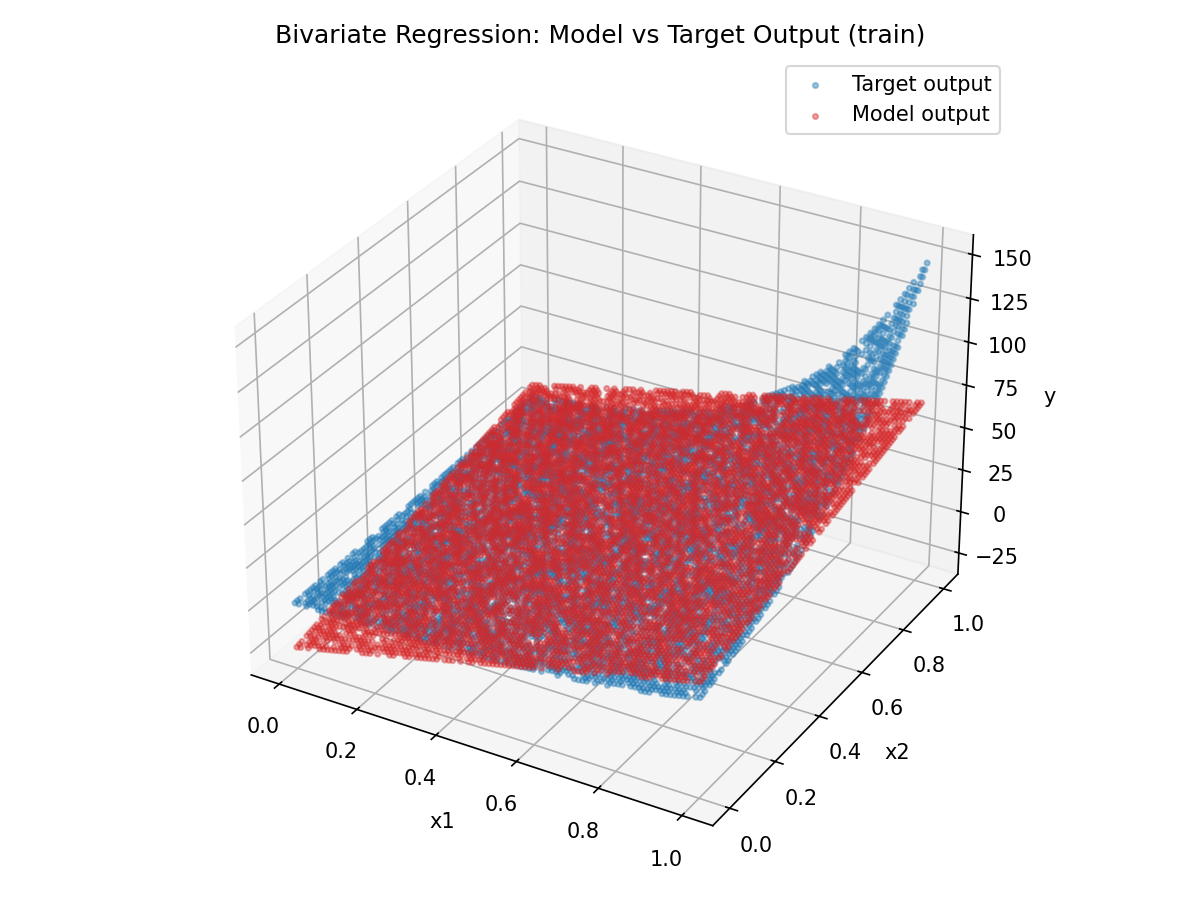
\includegraphics[width=\linewidth]{../regression_bivariate/model_vs_target_train.png}
\caption*{Training data}
\end{minipage}
\hfill
\begin{minipage}{0.48\textwidth}
\centering
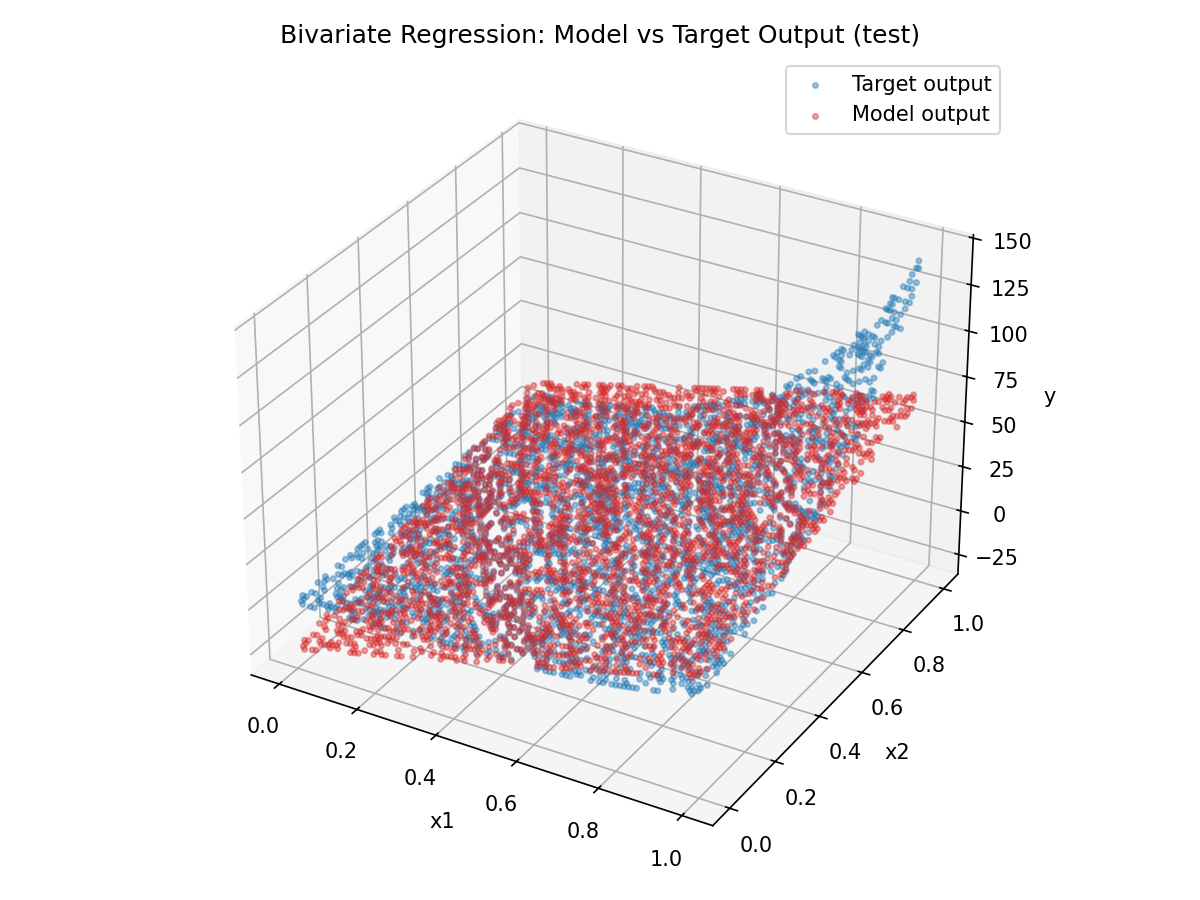
\includegraphics[width=\linewidth]{../regression_bivariate/model_vs_target_test.png}
\caption*{Test data}
\end{minipage}
\end{figure}

\begin{figure}[H]
\centering
\begin{minipage}{0.48\textwidth}
\centering
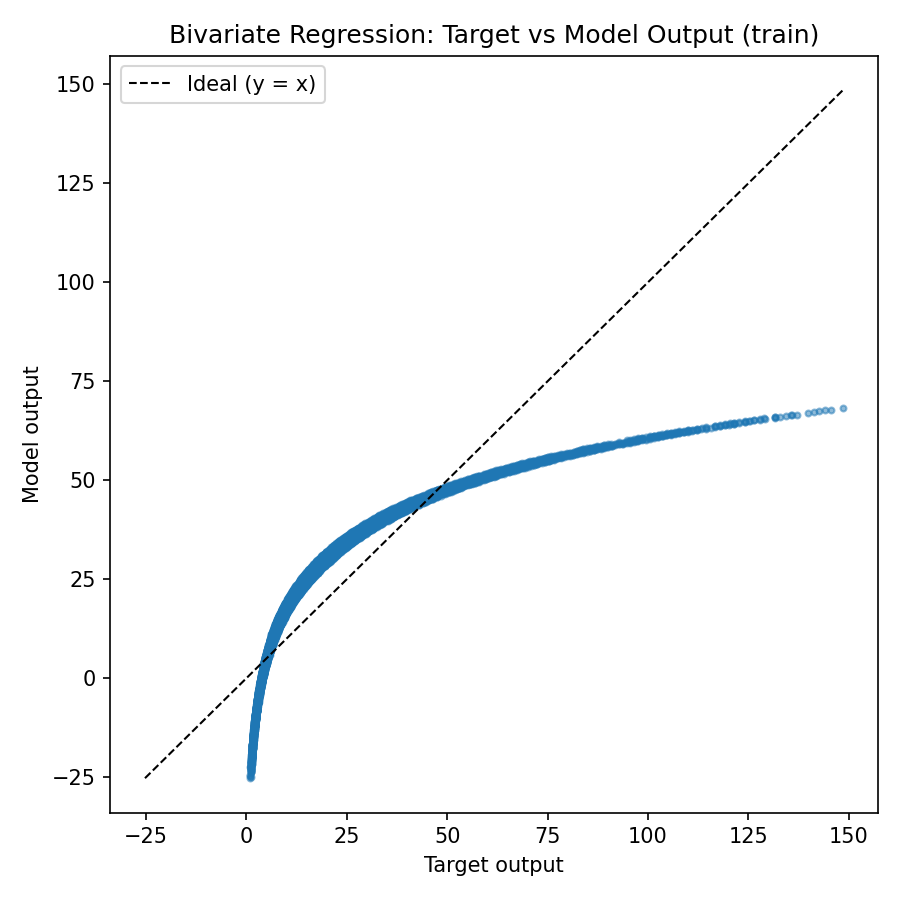
\includegraphics[width=\linewidth]{../regression_bivariate/scatter_target_vs_model_train.png}
\caption*{Training data}
\end{minipage}
\hfill
\begin{minipage}{0.48\textwidth}
\centering
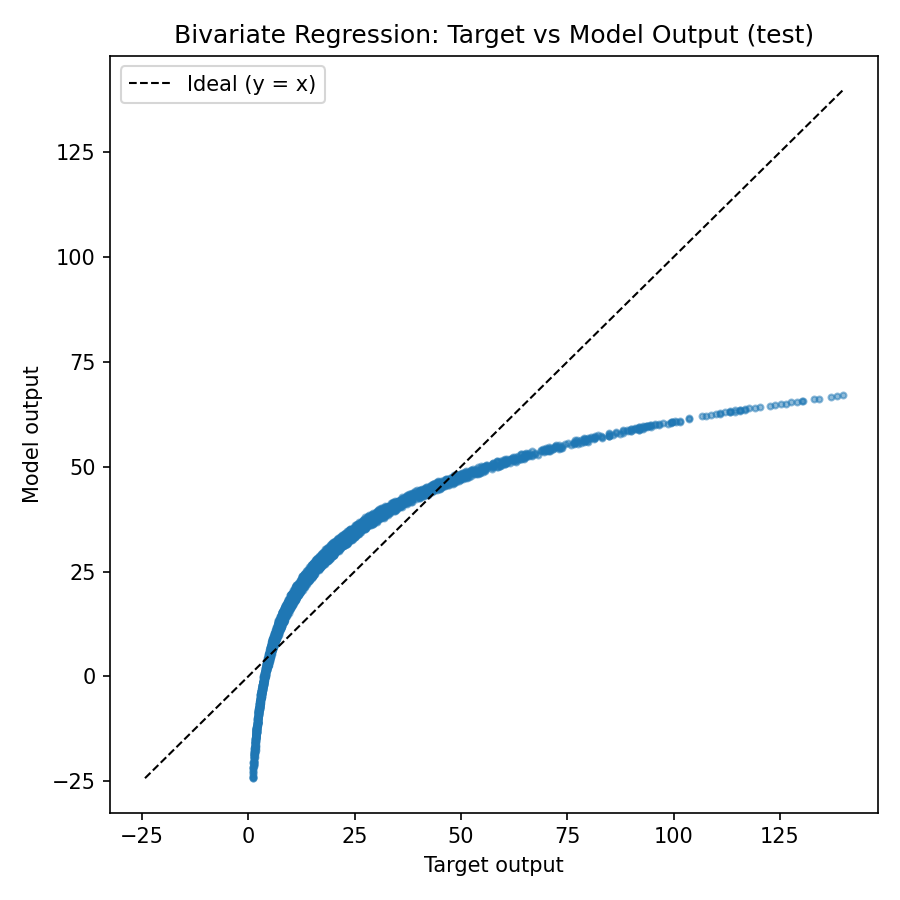
\includegraphics[width=\linewidth]{../regression_bivariate/scatter_target_vs_model_test.png}
\caption*{Test data}
\end{minipage}
\end{figure}
\clearpage

\section{Inferences and Observations}
\subsection{Classification}
On the \textbf{linearly separable (LS)} dataset, all three one-against-one perceptrons converge to an average error close to zero within a small number of epochs, and the combined decision regions cleanly separate the three classes with straight-line boundaries. This yields 100\% test accuracy, 100\% precision, recall and F-measure for every class, for both the logistic and tanh activation functions -- as expected, since the three classes are, by construction, separable by straight lines and a single perceptron per pair is sufficient to find such a boundary.

On the \textbf{non-linearly separable (NLS)} dataset, the three classes form curved, interleaved ``moon-shaped'' clusters that cannot be separated by straight lines. Because each pairwise perceptron can only learn a linear decision boundary, the combined classifier achieves a lower test accuracy of about 92.9\% for both activation functions, with Class 2 showing the lowest recall and F-measure since it is most often confused with its neighbours in the pairwise classifiers. The logistic and tanh activations produce almost identical accuracy and confusion patterns; the two activations differ mainly in their output range and in the shape of the error surface during training, but since both ultimately learn the same class of linear decision boundary, their final decision regions and test performance are very similar. This confirms that the performance gap between the LS and NLS datasets is caused by the linear nature of the perceptron's decision boundary rather than by the choice of activation function.

\subsection{Regression}
In both regression datasets the target output is a visibly non-linear function of the input(s): the univariate target follows a U-shaped (roughly quadratic, symmetric about the middle of the input range) curve, and the bivariate target grows in a curved, super-linear fashion with $x_1$ and $x_2$. Because the perceptron uses a linear activation function, it can only fit a straight line (univariate) or a flat plane (bivariate) to the data -- it has no way to represent curvature.

For the univariate case, the best linear fit is nearly flat, since the target is symmetric and rises on both sides of the input range; this gives a relatively high \%RMSE of around 42--44\% on training and test data. The bivariate case shows a similar pattern with an even higher \%RMSE of around 56--57\%, reflecting the stronger curvature of that target surface. In both cases the average-error-vs-epochs plot drops sharply within the first few epochs and then plateaus, showing that gradient descent quickly converges to the best possible linear fit -- the remaining error is not due to under-training but is an irreducible bias caused by using a linear model for a non-linear relationship. The scatter plots of target vs. model output further confirm this: the points form a roughly horizontal band far from the ideal $y=x$ line, consistent with the model consistently under/over-predicting for large deviations of the input from the middle of its range. Test-set RMSE and \%RMSE are close to the corresponding training-set values in both datasets, which shows the perceptron is not overfitting -- its limited capacity is simply insufficient to capture the non-linear trend in the data.
\clearpage

\section{Conclusion}
This assignment implemented the perceptron learning algorithm and its online gradient-descent training rule entirely from scratch, together with custom implementations of every evaluation metric used. Across four experiments -- one-against-one classification with logistic and tanh activations on linearly and non-linearly separable data, and linear-activation regression on univariate and bivariate data -- a consistent pattern emerges: whenever the true relationship between input and output is linear (or the classes are linearly separable), a single perceptron is entirely sufficient and achieves near-perfect performance. Whenever the true relationship is non-linear, a single perceptron is fundamentally limited by its linear decision boundary / linear output surface, and no amount of additional training epochs or change of activation function can close this gap. This directly motivates the use of multi-layer neural networks with non-linear hidden layers, which are able to combine multiple linear boundaries to approximate arbitrarily non-linear decision regions and regression surfaces.

\end{document}
